\documentclass[twoside]{article}
\usepackage{graphicx}
\usepackage[top=2.5cm,left=2.5cm,right=2.5cm,bottom=2.5cm,headsep=0.3in,headheight=1in]{geometry}
\usepackage{multirow}
\usepackage[ngerman]{babel}
\usepackage{float}
\usepackage{fancyhdr}
\usepackage{minted}
\usepackage{siunitx}


%Eingabe der Parameter in die letzten geschwungenen Klammern

\newcommand{\titeltitel}{Bluetooth}                  %Titel der Übung
\newcommand{\titelraumbezeichnung}{}        %Raumbezeichnung
\newcommand{\titelgruppe}{E}                 %Gruppe
\newcommand{\titellehrer}{LAP}                 %Lehrer
\newcommand{\titeluebungsnummer}{2}          %Übungsnummer
\newcommand{\titelabgabedatum}{24.01.2025}            %Abgabedatum
\newcommand{\titelkatalognummer}{25}          %Katalognummer
\newcommand{\titeluebungdatum}{17.01.2025}            %Übungsdatum
\newcommand{\titelnameprotokoll}{Reichart Florian}          %Name des Protokollist
\newcommand{\titelnameteam}{Mayer Phillip}               %Name der Teammitglieder
\newcommand{\titelklasse}{5BHEL}                 %Klasse
\newcommand{\titelgeprueftdatum}{}          %Prüfungsdatum  %Definiert Variablen für das Titelblatt

\begin{document}

%Titelblatt
\thispagestyle{empty}
\newgeometry{top=20mm, left=18.25mm, right=18.25mm, bottom=20mm}
\noindent
\begin{tabular}{|p{4.5cm}|p{7.5cm}|p{2.5cm}|p{2cm}|} %17.35mm
    \hline
    \vspace{0.4cm}
    \multirow{2}{4.5cm}{\hspace{0.7cm}
\includegraphics{img/titel/Labor_Protokoll_Logo.jpg}} & \multirow{2}{7.5cm}{\begin{center}{\huge Laboratorium}\\\vspace{0.25cm} Raumbezeichnung: \hspace{0.25cm} \titelraumbezeichnung \end{center}} & \vspace{0.05cm} Katalognummer:\vspace{0.3cm} & \vspace{0.06cm}\hspace{0.7cm}{\Large\titelkatalognummer}\\
    \cline{3-4}
     & & \vspace{0.05cm}Tag der Übung:\vspace{0.3cm} & \vspace{0.14cm} {\large\titeluebungdatum} \\
    \hline
    \vspace{0.35cm} {\large Gruppe: \titelgruppe} & \vspace{0.1cm} {Protokoll: \hspace{0.27cm} \titelnameprotokoll \vspace{0.1cm} \newline Mitglieder: \hspace{0.1cm} \titelnameteam} \vspace{0.2cm} & \vspace{0.35cm} {\large Klasse} & \vspace{0.35cm} {\Large\titelklasse} \\
    \hline
    \multicolumn{4}{|p{17cm}|}{
    \centering
    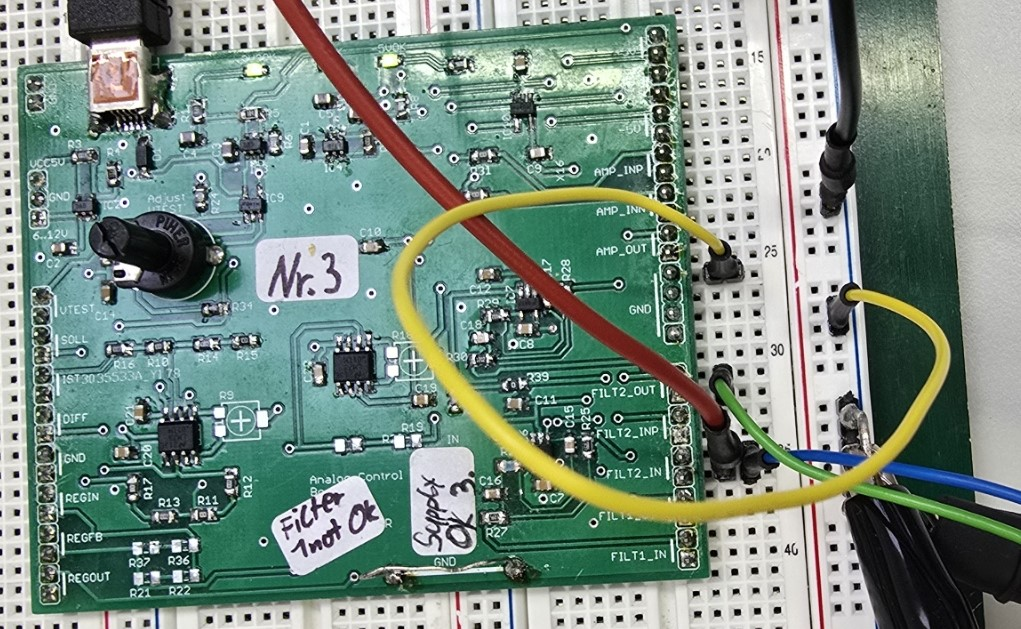
\includegraphics[width=0.85\linewidth]{img/Aufbau_03.jpg}
    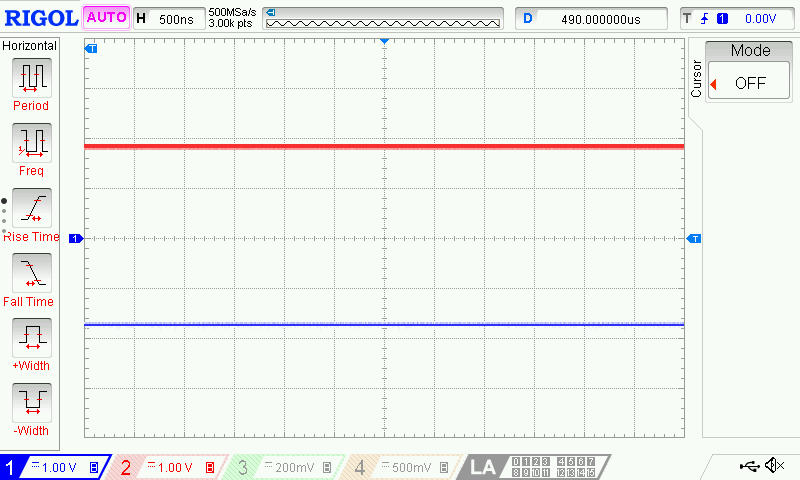
\includegraphics[width=0.85\linewidth]{img/Oszi_06.jpg}
    \vspace{0.1cm}}\\
    \hline
\end{tabular}

\vspace{-1px}
\noindent
\begin{tabular}{|p{2.3cm}|p{1.8cm}|p{7.9cm}|p{2.5cm}|p{1.58cm}|}
    \vspace{0.1cm}Lehrer\vspace{0.2cm} & \vspace{0.1cm}\titellehrer & \vspace{0.15cm} \multirow{2}{7.1cm}{\centerline{Titel der Übung}\vspace{0.2cm}\newline\centerline{\huge \textbf{\titeltitel}}} & \vspace{0px} Übungsnummer & \vspace{1px}\titeluebungsnummer\\
    \cline{1-2}\cline{4-5}
    \vspace{0px}Geprüft\vspace{0.15cm} & \vspace{0px} \titelgeprueftdatum &  & \vspace{0px}Abgabe am\vspace{0.15cm} & \vspace{0px}\titelabgabedatum \\
    \hline
\end{tabular}
\newgeometry{top=2.5cm,left=2.5cm,right=2.5cm,bottom=2.5cm,headsep=0.3in,headheight=1in}

%Kopf- und Fußzeile
\pagestyle{fancy}
\fancyhead[R]{\titelnameprotokoll} %Protokollist oben rechts
\fancyhead[L]{\titeluebungdatum}   %Übungsdatum oben links
\fancyfoot[C]{\titeltitel}         %Titel der Übung unten mittig
\fancyfoot[R]{\thepage}           %Seitennummer unten außen

%Inhaltsverzeichnis
\tableofcontents
\newpage

%Begin der Dokumentation
\section{Inbetriebnahme der Regler-Platine}
\subsection{Aufgabenstellung}
In dieser Aufgabe soll die Regler-Platine (Modul Nummer: 3) ohne Beschaltung in Betrieb genommen werden. Dabei sollen die Versorgungsspannungen sowie der Spannungsbereich von $V_{test}$ überprüft werden.

\subsection{Kontrolle der Versorgungsspannung}
Um die Versorgungsspannung zu überprüfen, wurde die Regler-Platine über den USB-Port an 5V angeschlossen. Aus der Messung folgte ein Spannungswert von \textbf{5.08V}.
\begin{figure}[h]
    \centering
    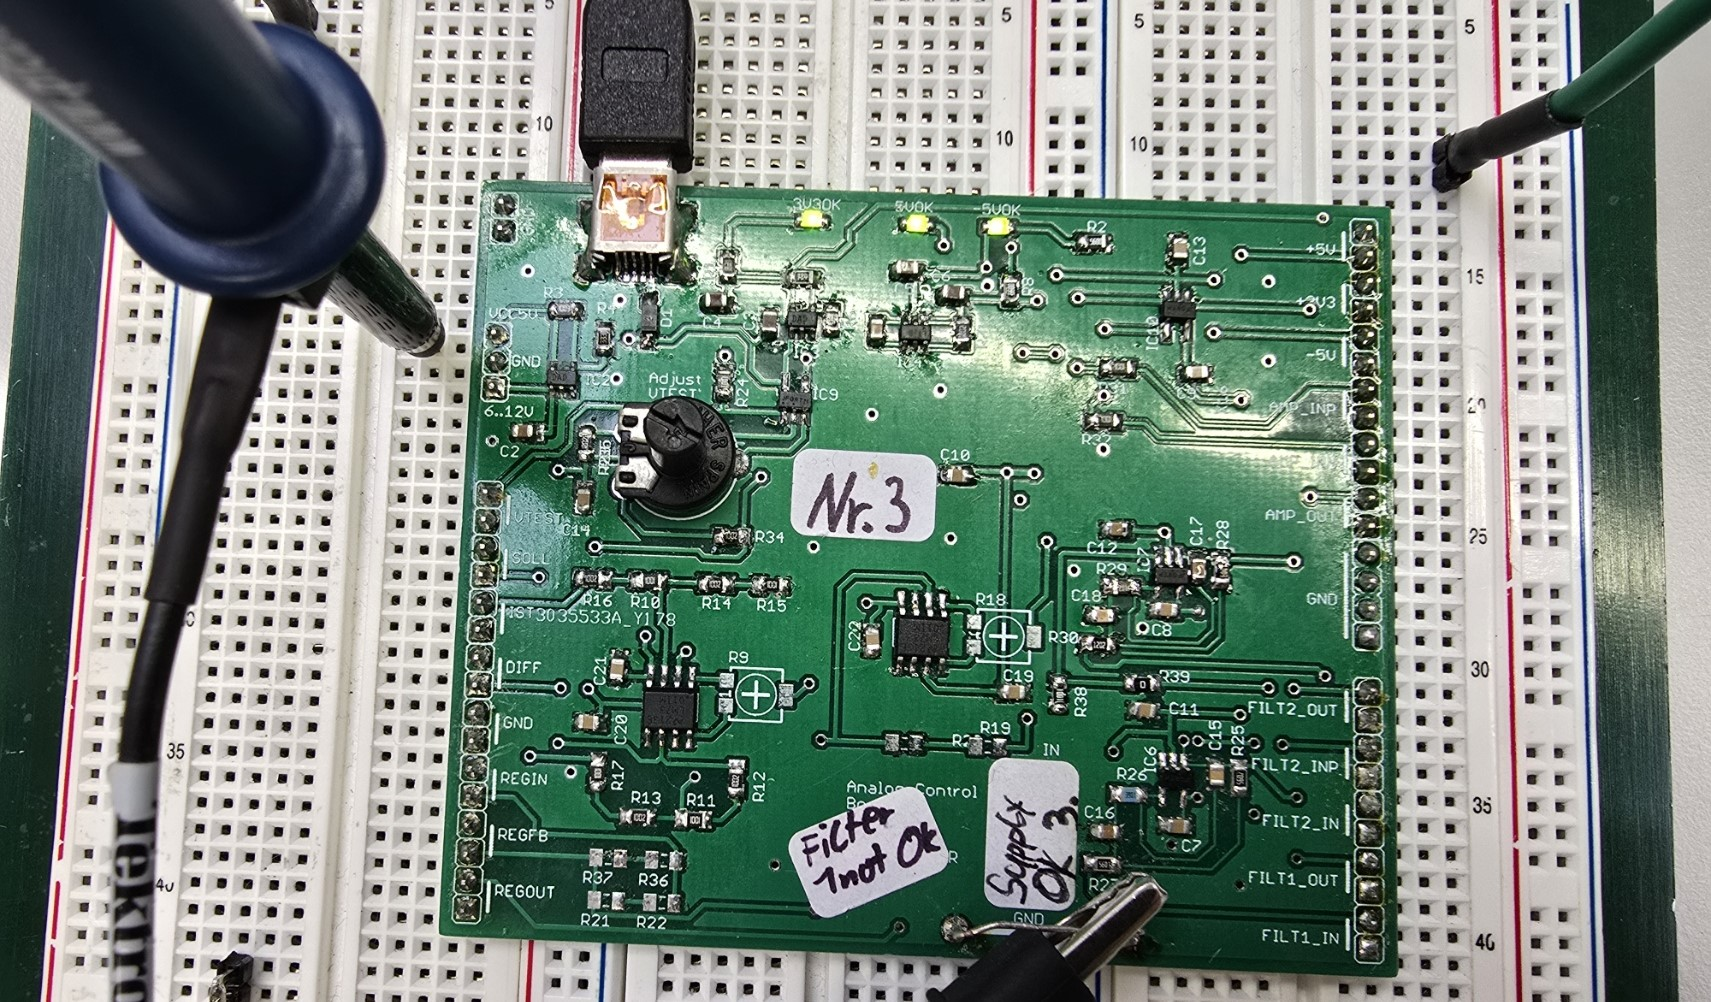
\includegraphics[width=0.75\linewidth]{img/Aufbau_01.jpg}
\end{figure}

\subsection{Kontrolle der Testspannung}
Für die Messung des Bereiches der Testspannung wurde das Potentiometer, welches die Spannung des Punktes kontrolliert, an beide Limits eingestellt und es wurde gemessen, welche Spannungen somit maximal bzw. minimal eingestellt werden können. Dabei wurde ein Spannungsbereich von -1.68 V ... +1.8 V gemessen.
\begin{figure}[h]
    \centering
    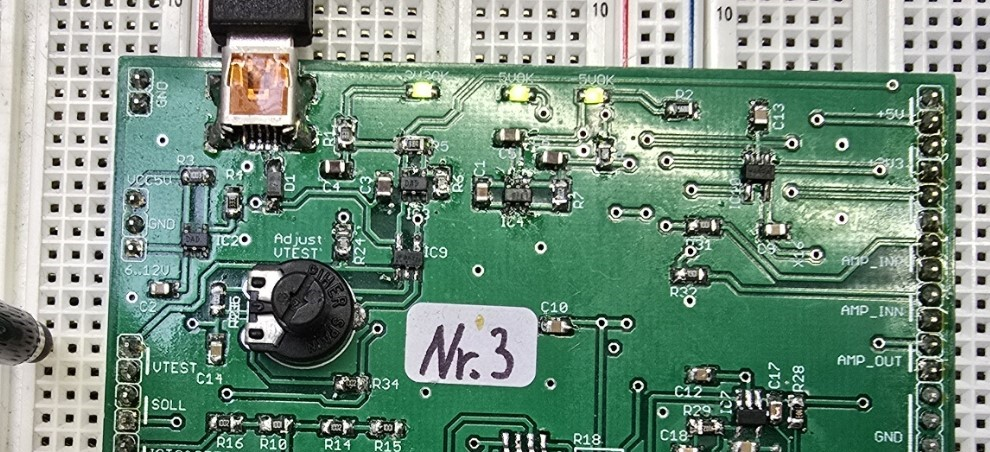
\includegraphics[width=0.75\linewidth]{img/Aufbau_02.jpg}
\end{figure}
-1.68V ... +1.8 V

\newpage
\section{Kontrolle der Regeldifferenz}
\subsection{Aufgabenstellung}
In dieser Aufgabe soll die korrekte Funktionsweise des Regeldifferenz überprüft werden. Dafür soll die Offset-Spannung aufgenommen werden und verschiedene Messpunkte zur Bestimmung der korrekten Funktionsweise.

\subsection{Kontrolle der Offset-Spannung}
Für die Messung der Offset-Spannung wurden beide Eingänge des Subtrahierers auf GND gelegt. Dabei wurde eine Offset-Spannung von ca. \textbf{2 mV} erfasst.

\subsection{Kontrolle des Subtrahierers}
Für die Messung der richtigen Funktion der Schaltung wurde ein Eingang auf GND und der andere Eingang auf $V_{test}$ gelegt. Da das Ausgangssignal den negativen Wert der $V_{test}$-Spannung hatte, konnte die korrekte Funktion belegt werden. Dies wurde durch Messungen bei mehrere Spannungen bestätigt.
\begin{figure}[h]
\centering
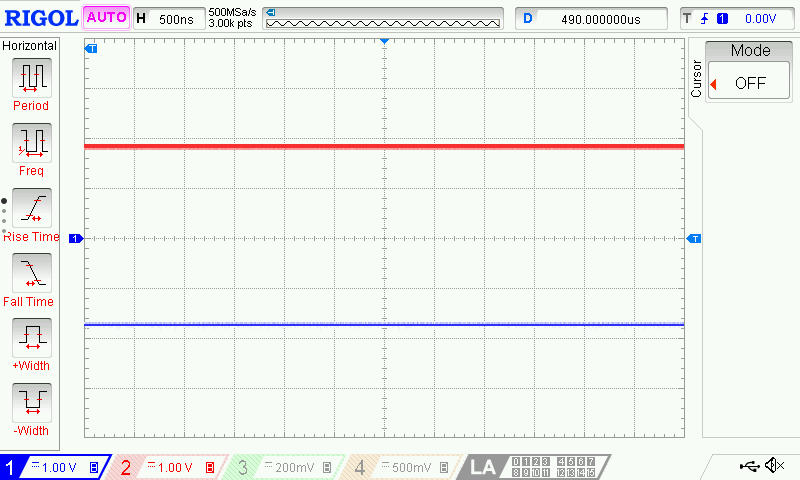
\includegraphics[width=0.75\linewidth]{img/Oszi_06.jpg}
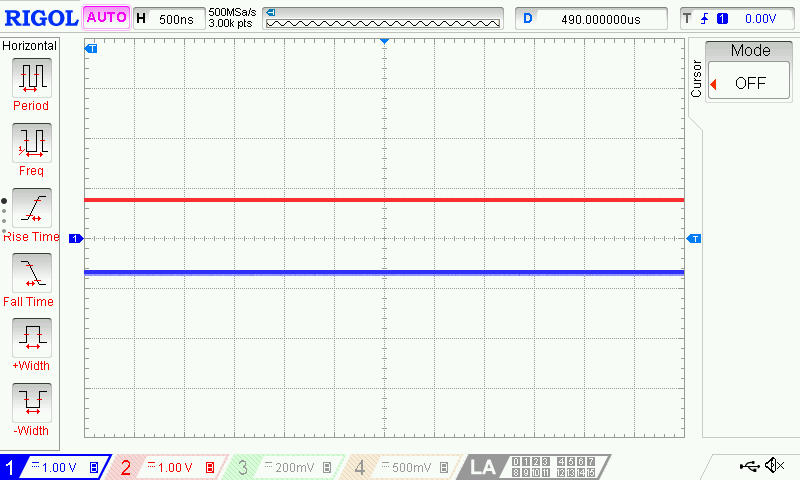
\includegraphics[width=0.75\linewidth]{img/Oszi_07.jpg}
\end{figure}

\newpage
\section{Aufnahme der Streckensprungantwort}
\subsection{Aufgabenstellung}
In dieser Aufgabe soll die Sprungantwort der künstlichen Strecke messtechnisch aufgenommen werden. Dazu soll am Eingang der Strecke ($FLT2_{IN}$) mit einem Funktionsgenerator ein Sprung (Rechtecksignal) angelegt werden. Die resultierende Sprungantwort kann anschließend mit einem Oszilloskop am Ausgang der Strecke ($FLT2_{OUT}$) aufgenommen werden.

\subsection{Messaufbau}
\begin{figure}[h]
    \centering
    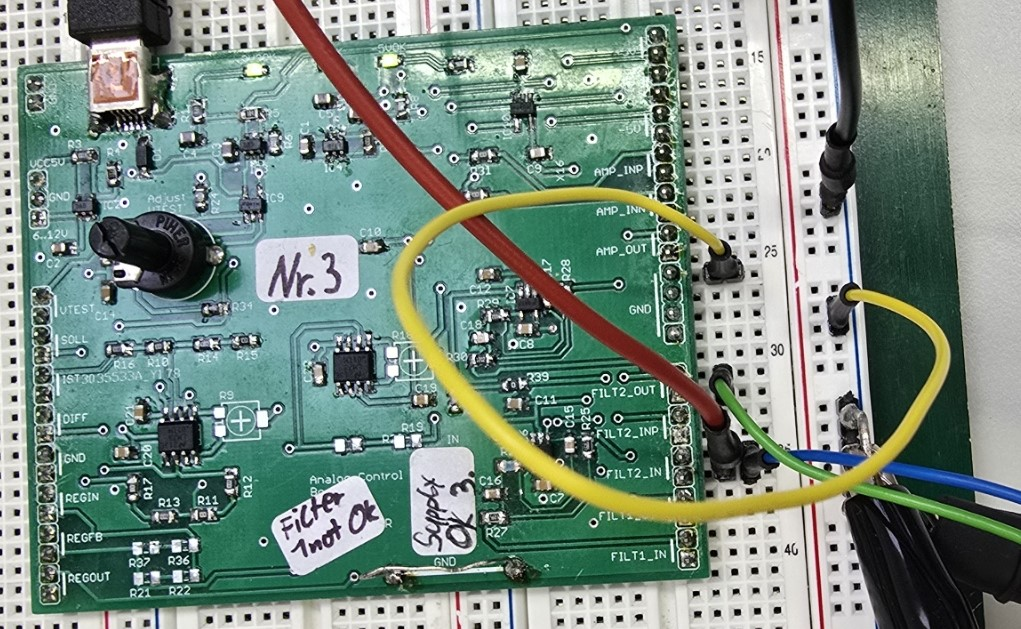
\includegraphics[width=0.75\linewidth]{img/Aufbau_03.jpg}
\end{figure}

\subsection{Streckensprungantwort}
\begin{figure}[h]
    \centering
    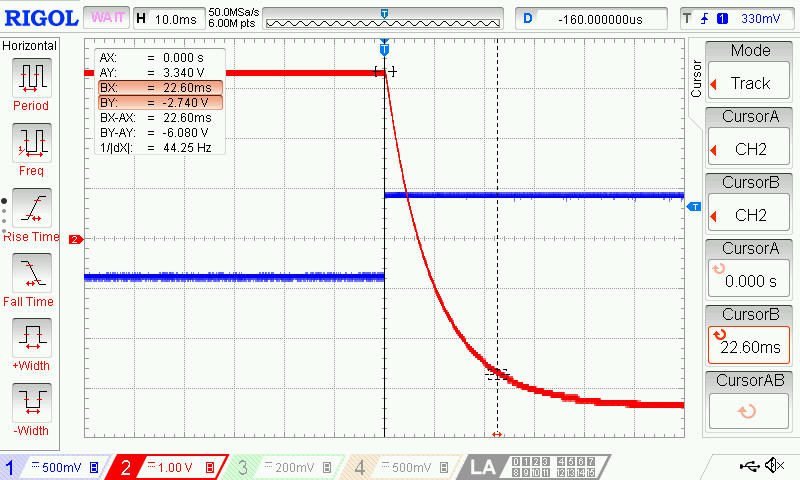
\includegraphics[width=0.75\linewidth]{img/Messung_01.png}
\end{figure}

\newpage
\section{Übertragungsfunktion der Strecke}
\subsection{Aufgabenstellung}
In dieser Aufgabe soll die zuvor ermittelte Messung genutzt werden, um die Übertragungsfunktion (G(s)) der Strecke zu bilden. Dafür müssen die drei Punkte $t_{10}$, $t_{50}$ und $t_{90}$ aus der Sprungantwort abgelesen werden.

\subsection{Bestimmung der Messpunkte}
Die drei Messpunkte $t_{10}$, $t_{50}$ und $t_{90}$ sind die Zeitpunkte, an denen das Signal 10\%, 50\% und 90\% seines maximalen Wertes erreicht. Da die Sprungantwort von 3.35 V auf -3.38 V abfällt, ist die maximale Änderung der Sprungantwort -6.72 V. Der folgende Matlab-Code berechnet die gesuchten Spannungen für die Messpunkte:
\begin{minted}{matlab}
dVa=-6.72;      % maximale Änderung der Sprungantwort

vt10=0.1*dVa    % Spannungänderung bei t10
vt50=0.5*dVa    % Spannungänderung bei t50
vt90=0.9*dVa    % Spannungänderung bei t90
\end{minted}

\subsection{Messung der Messpunkte}
Über die zuvor bestimmten Spannungsänderungen konnten die Zeitpunkte für $t_{10}$, $t_{50}$ und $t_{90}$ bestimmt werden.\\\\
\begin{tabular}{ l l }
    $t_{10}$ & 1.2 ms \\
    $t_{50}$ & 6.8 ms \\
    $t_{90}$ & 20 ms \\
\end{tabular}

\subsection{Bestimmung der Übertragungsfunktion}
Durch die gemessenen Zeitpunkte $t_{10}$, $t_{50}$ und $t_{90}$ sowie die Verstärkung K der Sprungantwort kann die Übertragungsfunktion eines Systems ausgerechnet werden. Dafür müssen die Werte Alpha und Beta aus zwei Graphen bestimmt werden.\\\\
\begin{tabular}{ l l }
    Alpha & 28 \\
    Beta & 3.4 \\
\end{tabular}

Aus diesen Werten können die zwei benötigten Grenzfrequenzen berechnet werden.
\begin{minted}{matlab}
fg2=Beta/t50
fg1=fg2/Alpha

T1=1/(fg1*2*pi)
T2=1/(fg2*2*pi)
\end{minted}

\begin{tabular}{l l}
    $f_{g1}$ & 500 Hz \\
    $f_{g2}$ & 17.8571 Hz \\
    $T_{1}$ &  8.9 ms\\
    $T_{2}$ &  0.3183 ms\\
\end{tabular}

Somit lautet die Übertragungsfunktion der Strecke wie folgt:
\begin{equation}
    G(s) = \frac{K}{\left(\frac{s}{f_{g1}} + 1\right)\left(\frac{s}{f_{g2}} + 1\right)}
\end{equation}
\newpage
\subsection{Bodediagramm}\mbox{}\\
\begin{figure}[h]
    \centering
    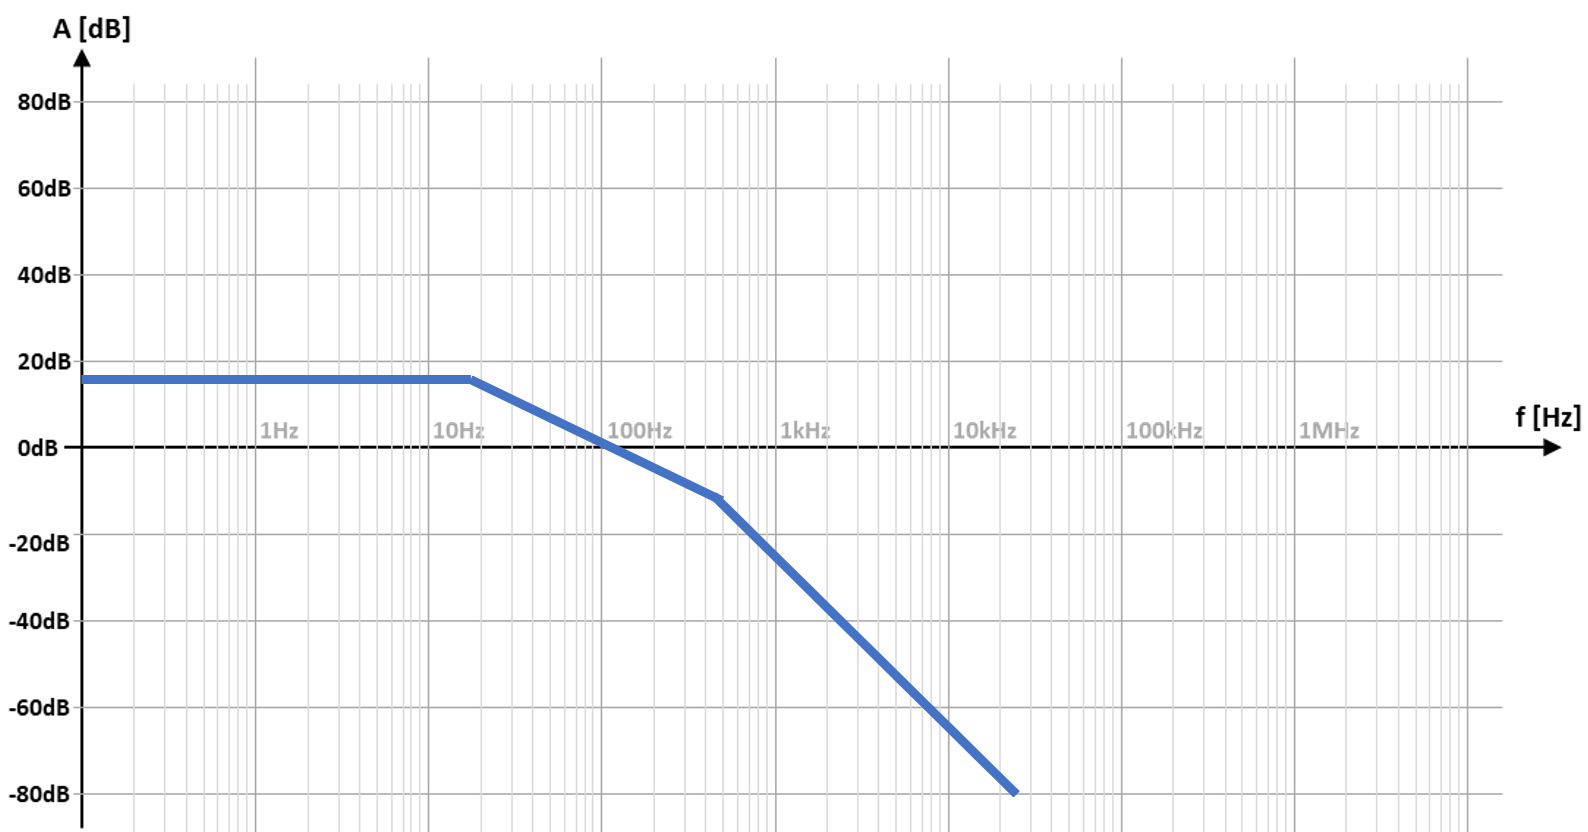
\includegraphics[width=0.9\linewidth]{img/Bode_01.png}
\end{figure}
\begin{figure}[h]
    \centering
    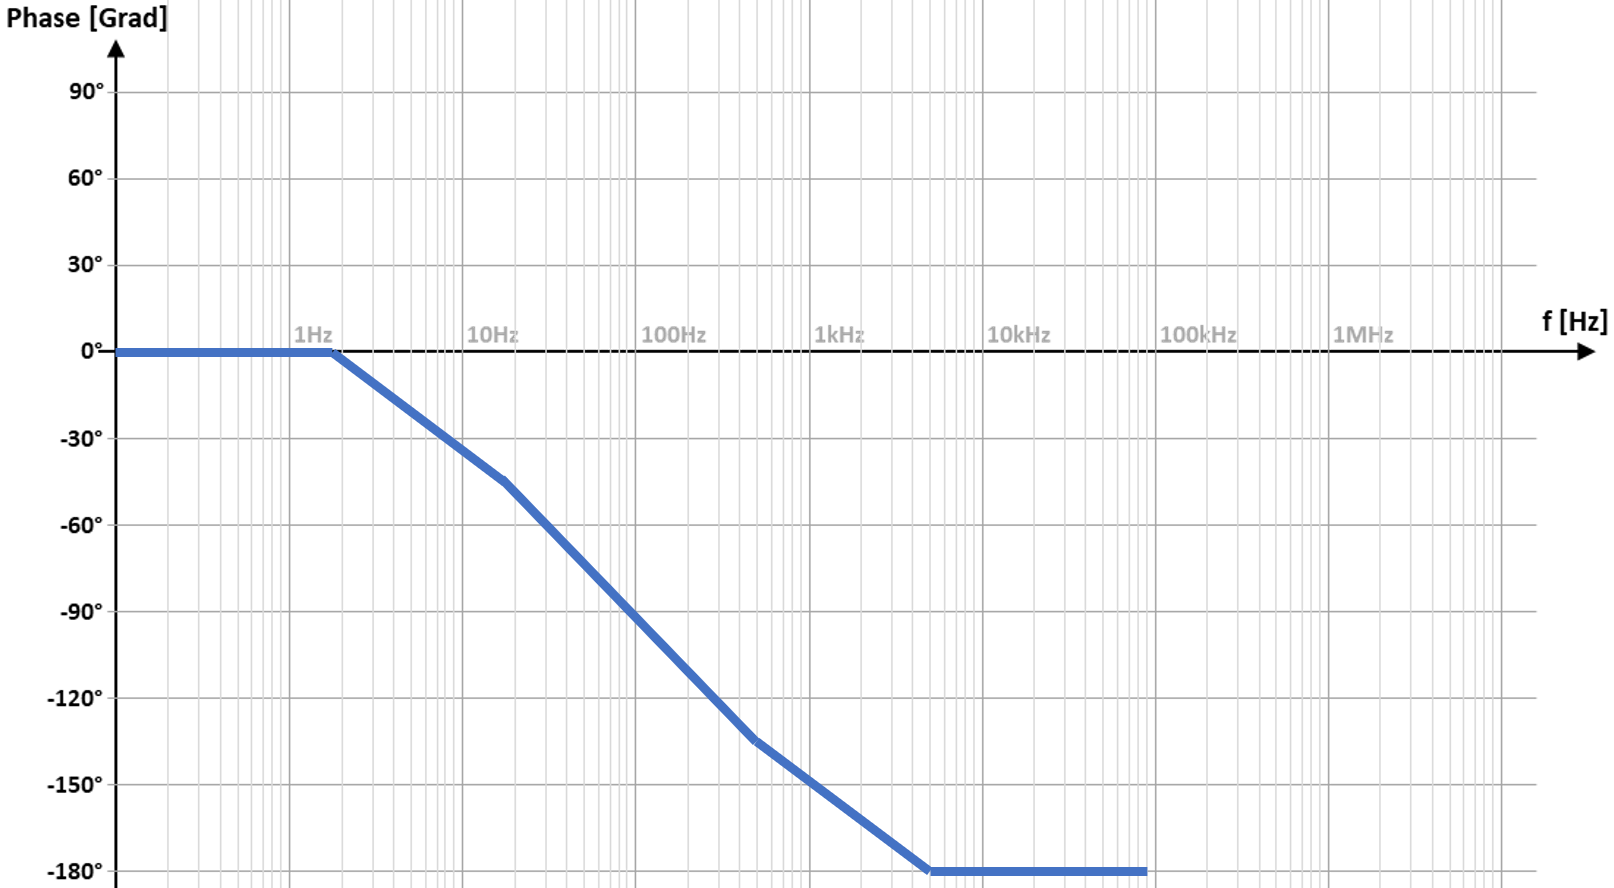
\includegraphics[width=0.9\linewidth]{img/Bode_02.png}
\end{figure}

\newpage
\section{Nachbildung der Strecke}
\subsection{Aufgabenstellung}
In dieser Aufgabe soll die zuvor berechnete Übertragungsfunktion der Strecke in Matlab nachgebildet werden.

\subsection{Matlab-Code}
\begin{minted}{matlab}
s = tf('s')
Gs= K/((s/fg1+1)*(s/fg2+1))
bode(Gs)
\end{minted}

\subsection{Erhaltener Graph}
\begin{figure}[h]
    \centering
    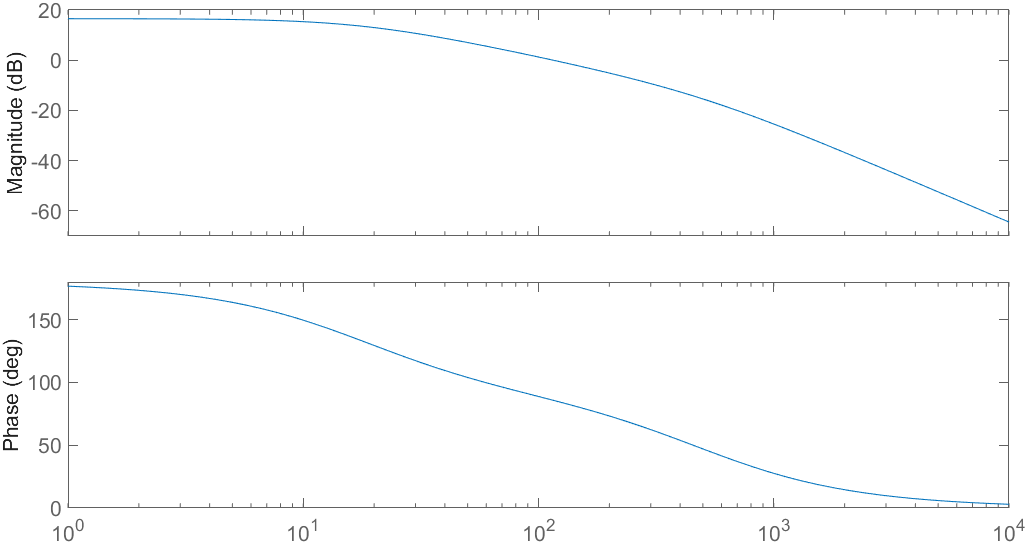
\includegraphics[width=1\linewidth]{img/Bode_03.png}
\end{figure}

\subsection{Vergleich}
Beim Vergleich der beiden Bodediagramme ist erkennbar, dass beide Graphen bei ca. 18 dB starten. Bei einer Frequenz von ca. 17.2 Hz ist die Verstärkung des Graphen um -3 dB vom Maximum gefallen. Zudem beträgt die Verstärkung der Simulation bei der Frequenz von 500 Hz ca. -14 dB. Dieser Wert passt sehr gut zu dem gezeichneten Graphen, bei dem bei 500 Hz eine Verstärkung von ca. -15 dB ausgelesen werden kann.\\
Auch die Phasengänge des gezeichneten und simulierten Bodediagramms passen gut zusammen, aber es kann eine leichte Abweichung zwischen den beiden Grenzfrequenzen festgestellt werden, da der Phasengang der Simulation an dieser Stelle flacher verläuft, wie im selbst gezeichneten Diagramm. 

\newpage
\section{I-Regler}
\subsection{Aufgabenstellung}
In dieser Aufgabenstellung soll ein I-Regler entworfen werden, der nach dem Phasenrandkriterium ein Überschwingen von 10\% verursacht.

\subsection{Berechnung des Phasenrands}
Um den I-Regler zu dimensionieren, muss zuerst der Phasenrand mithilfe des Überschwingens berechnet werden.
\begin{equation}
\varphi_{r} = 70° - \ddot u = 70° - 10° = 60°
\end{equation}

\subsection{Entwurf des I-Reglers}
Die Verstärkung eines I-Reglers fällt um 20 dB / Dekade und muss im Bodediagramm so platziert werden, dass beim Frequenzpunkt, an dem das Phasenrandkriterium erfüllt ist, die Summe des Reglers und der Strecke 1 (0 dB) ist. Somit ist die Verstärkung des I-Reglers am Punkt des Phasenrandkriteriums der Kehrwert (linear) bzw. der negative Wert (logarithmisch) der Strecke.

\subsection{Bodediagramm}
\begin{figure}[h]
    \centering
    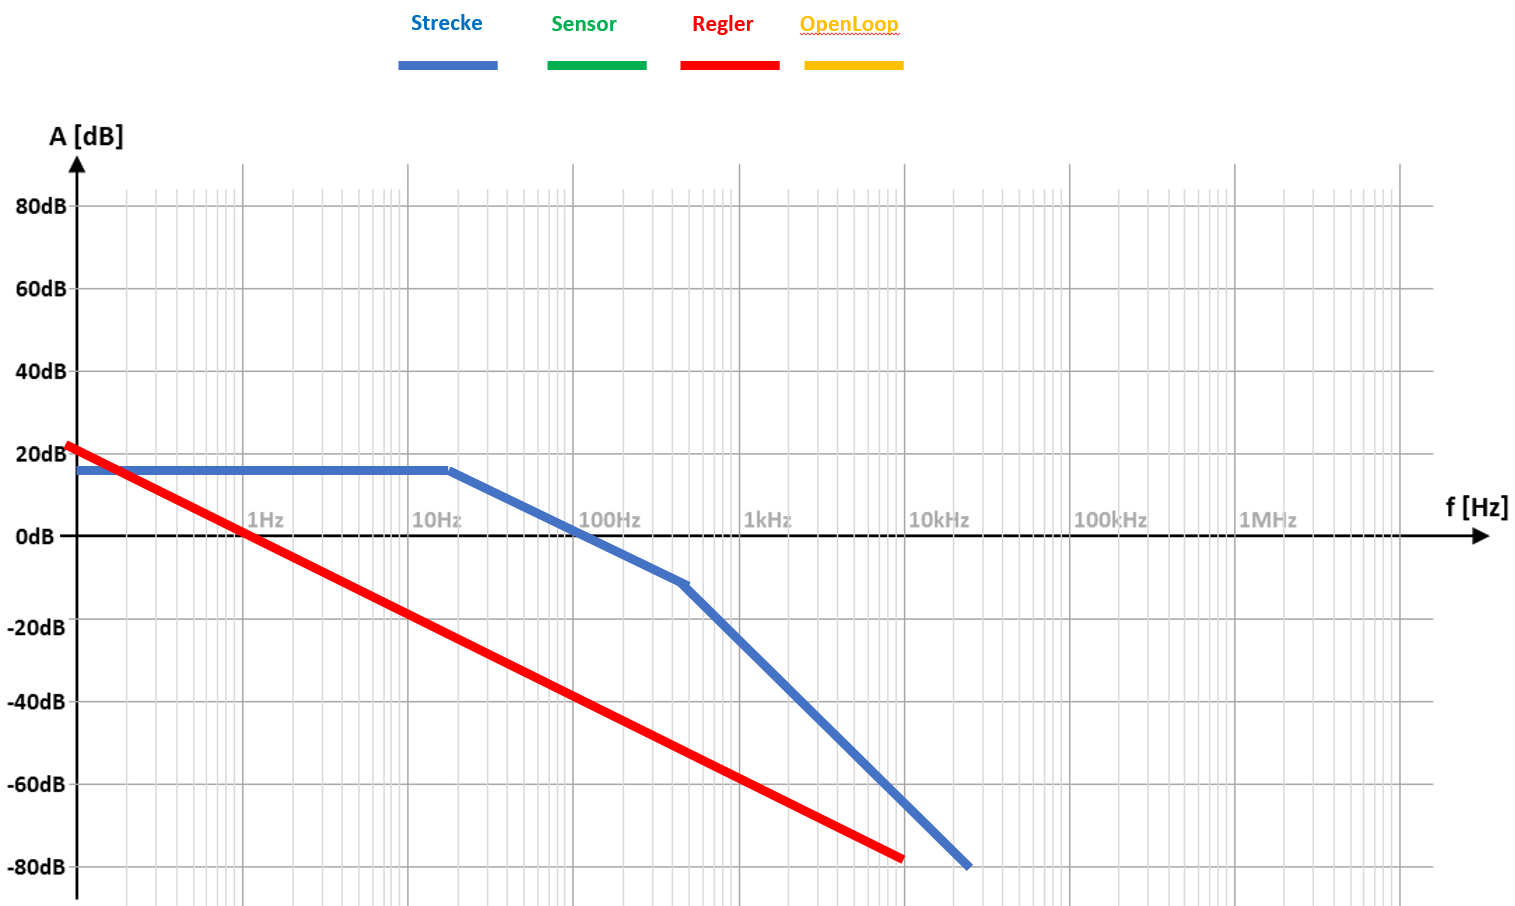
\includegraphics[width=1\linewidth, height = 6cm]{img/Bode_04.png}
\end{figure}
\begin{figure}[h]
    \centering
    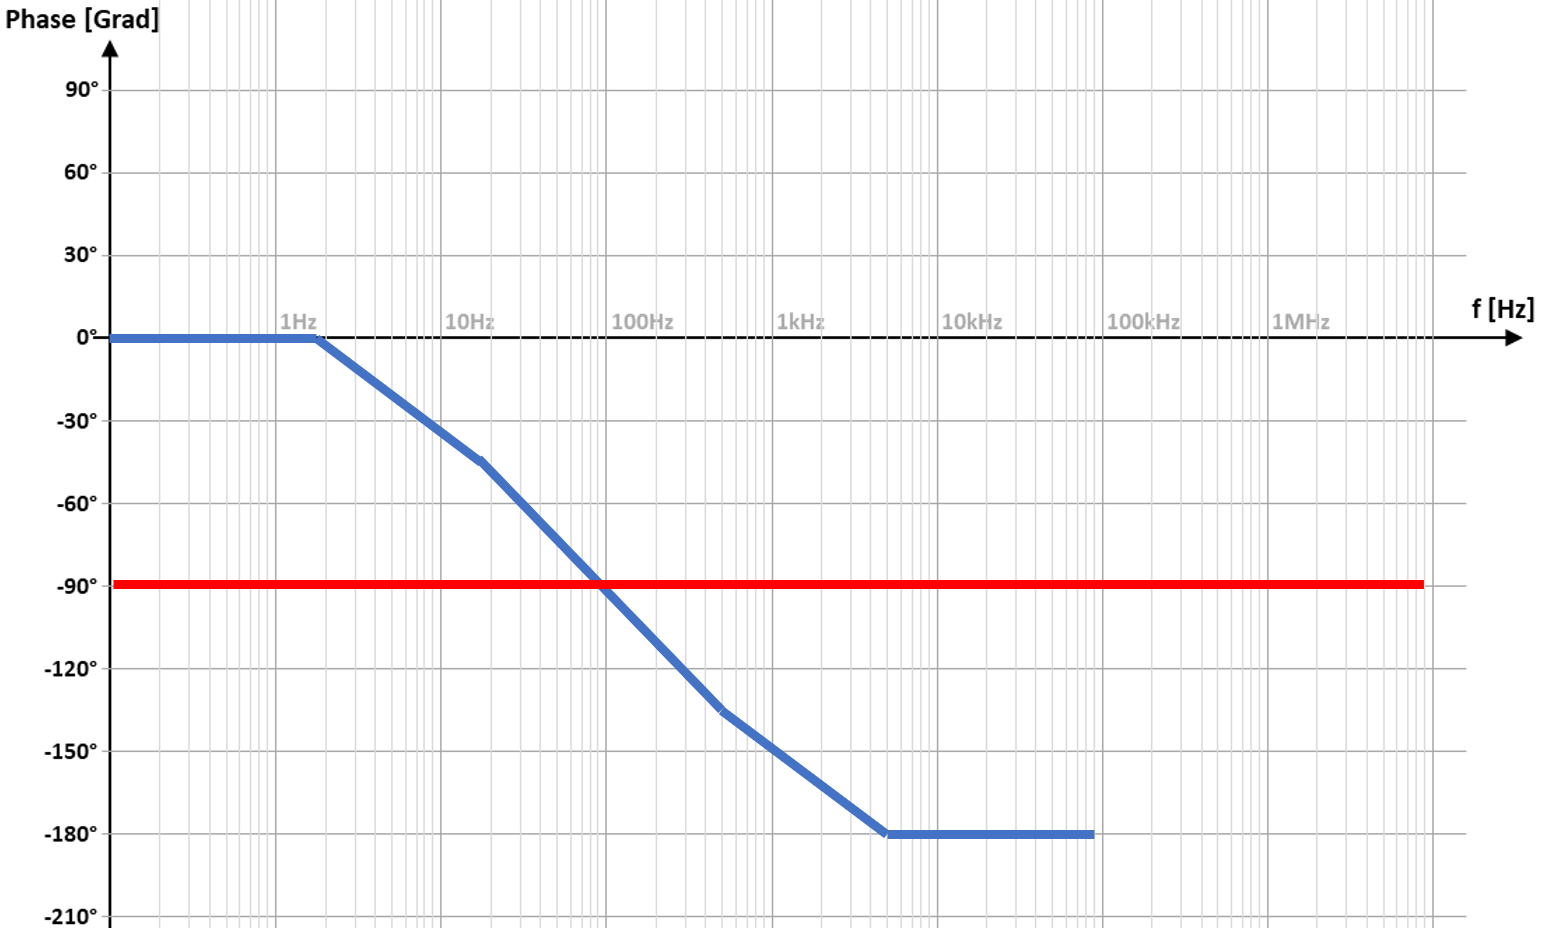
\includegraphics[width=1\linewidth, height = 6cm]{img/Bode_05.png}
\end{figure}

\subsection{Bestimmung des I-Faktors}
Für die Bestimmung des I-Faktors ($K_i$) muss die Durchtrittsfrequenz des Reglers bestimmt werden. Laut dem Bodediagramm ist diese ca. 1 Hz.
\begin{equation}
K_i=2\cdot \pi \cdot f_x
\end{equation}
\noindent
\textbf{Berechnung über Matlab}
\begin{minted}{matlab}
fx = 1;          % Durchtrittsfrequenz
Gx = 1;          % Verstärkung bei der Frequenz
Ki = 2*pi*fx*Gx  % I-Faktor
\end{minted}
Dabei wurde ein Ki-Wert von \textbf{6.2832} berechnet.
\newpage
\section{Überprüfung des Reglerverhaltens}
\subsection{Aufgabenstellung}
In dieser Aufgabe soll das Verhalten des erstellten I-Reglers mit Matlab überprüft werden.

\subsection{Reglerverhalten in Matlab}
\begin{minted}{matlab}
%Reglerverhalten
Gr = Ki/(s)
bode(Gr)
\end{minted}
\begin{figure}[h]
    \centering
    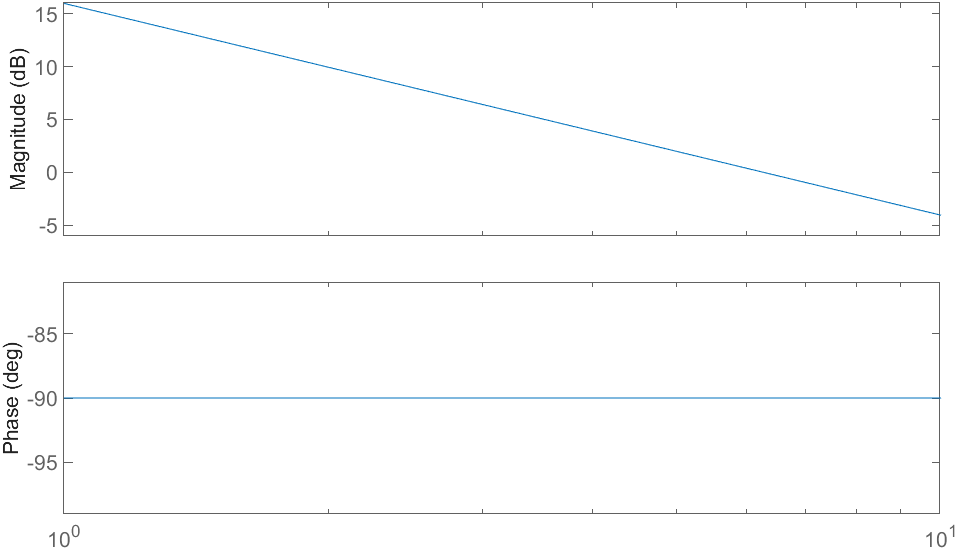
\includegraphics[width=1\linewidth]{img/Bode_06.png}
\end{figure}

\newpage
\section{Umsetzung des Reglers}
\subsection{Aufgabenstellung}
In dieser Aufgabe soll der Regler als Schaltung realisiert und aufgebaut werden.

\subsection{Schaltung}
Da ein I-Element ein Integrator ist, ist die Schaltung des I-Wandlers eine Integratorschaltung mit einem Operationsverstärker.
\begin{figure}[h]
    \centering
    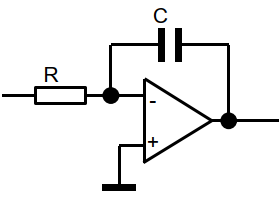
\includegraphics[width=1\linewidth]{img/Schaltung_01.png}
\end{figure}

\subsection{Berechnung der Bauteile}
Für die Schaltung des I-Wandlers werden die Werte für R und C benötigt. Da es eine größere Auswahl an Widerständen als bei Kondensatoren gibt, wurde der Kondensatorwert als \SI{1}{\micro\farad} angenommen und der Widerstand wurde berechnet.
\begin{equation}
R=\frac{1}{K_i \cdot C} = \frac{1}{6.2832 \cdot 1\cdot 10^{-6}}=159.15\ k\Omega
\end{equation}

\subsection{Wahl der Bauteile}
Da kein $160k\Omega$ verfügbar war, wurde ein $150k\Omega$ benutzt, um die Schaltung zu realisieren.
\newpage
\section{Test des Reglers}
\subsection{Aufgabenstellung}
In dieser Aufgabe soll der I-Wandler ohne Beschaltung getestet werden. Dafür soll eine Spannung an den Eingang des Reglers angelegt werden. Bei einer positiven Spannung sollte der Regler an das positive Rail des OPs stoßen.

\subsection{Positive Spannung}
Beim Anlegen einer positiven Spannung steigt die Ausgangsspannung rasch auf und stößt anschließend auf einen Maximalwert, der das Rail des OPs darstellt. Da dies der Theorie entspricht, ist die korrekte Funktion des Wandlers bestätigt.
\begin{figure}[h]
    \centering
    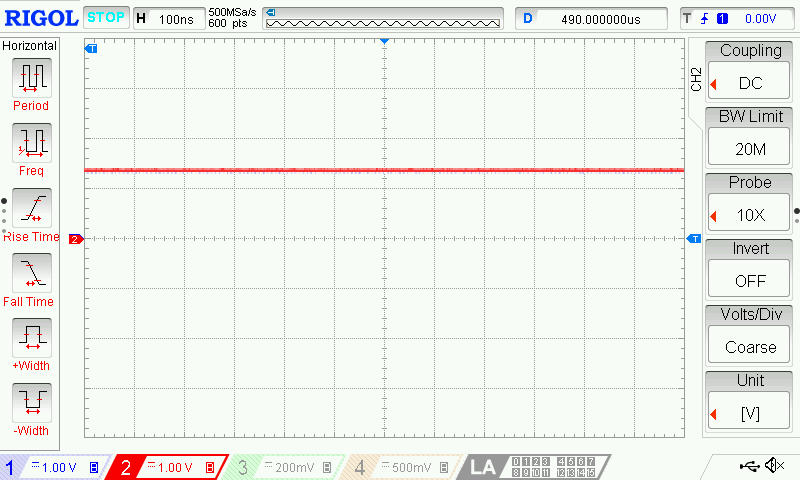
\includegraphics[width=1\linewidth]{img/Oszi_01.jpg}
\end{figure}

\newpage
\section{Test des Regelkreises}
\subsection{Aufgabenstellung}
In dieser Aufgabe soll die Funktion des gesamten Regelkreises überprüft werden. Dafür wird am Eingang ein Rechtecksignal angelegt und das Ausgangssignal wird untersucht.

\subsection{Bodediagramm}
\begin{figure}[h]
    \centering
    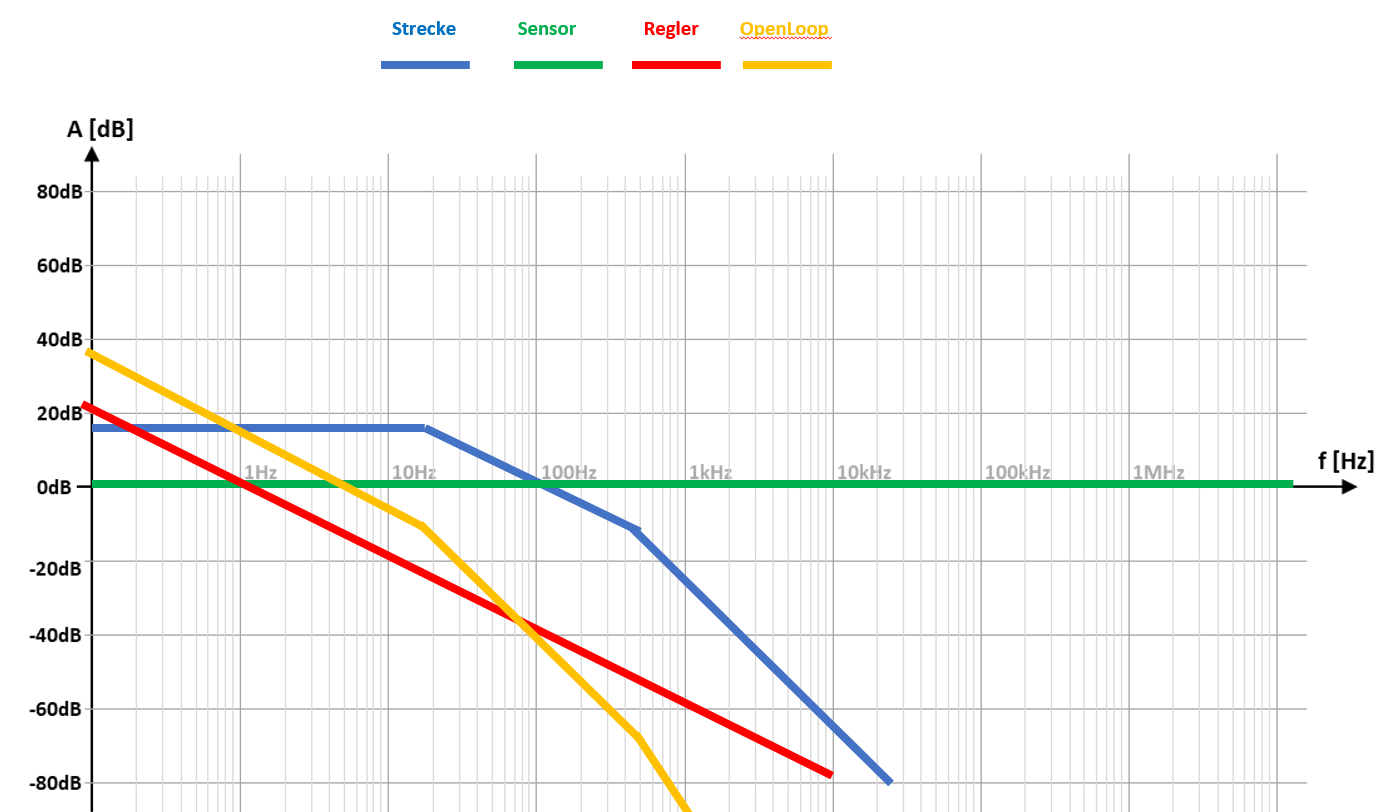
\includegraphics[width=1\linewidth, height=9cm]{img/Bode_07.png}
    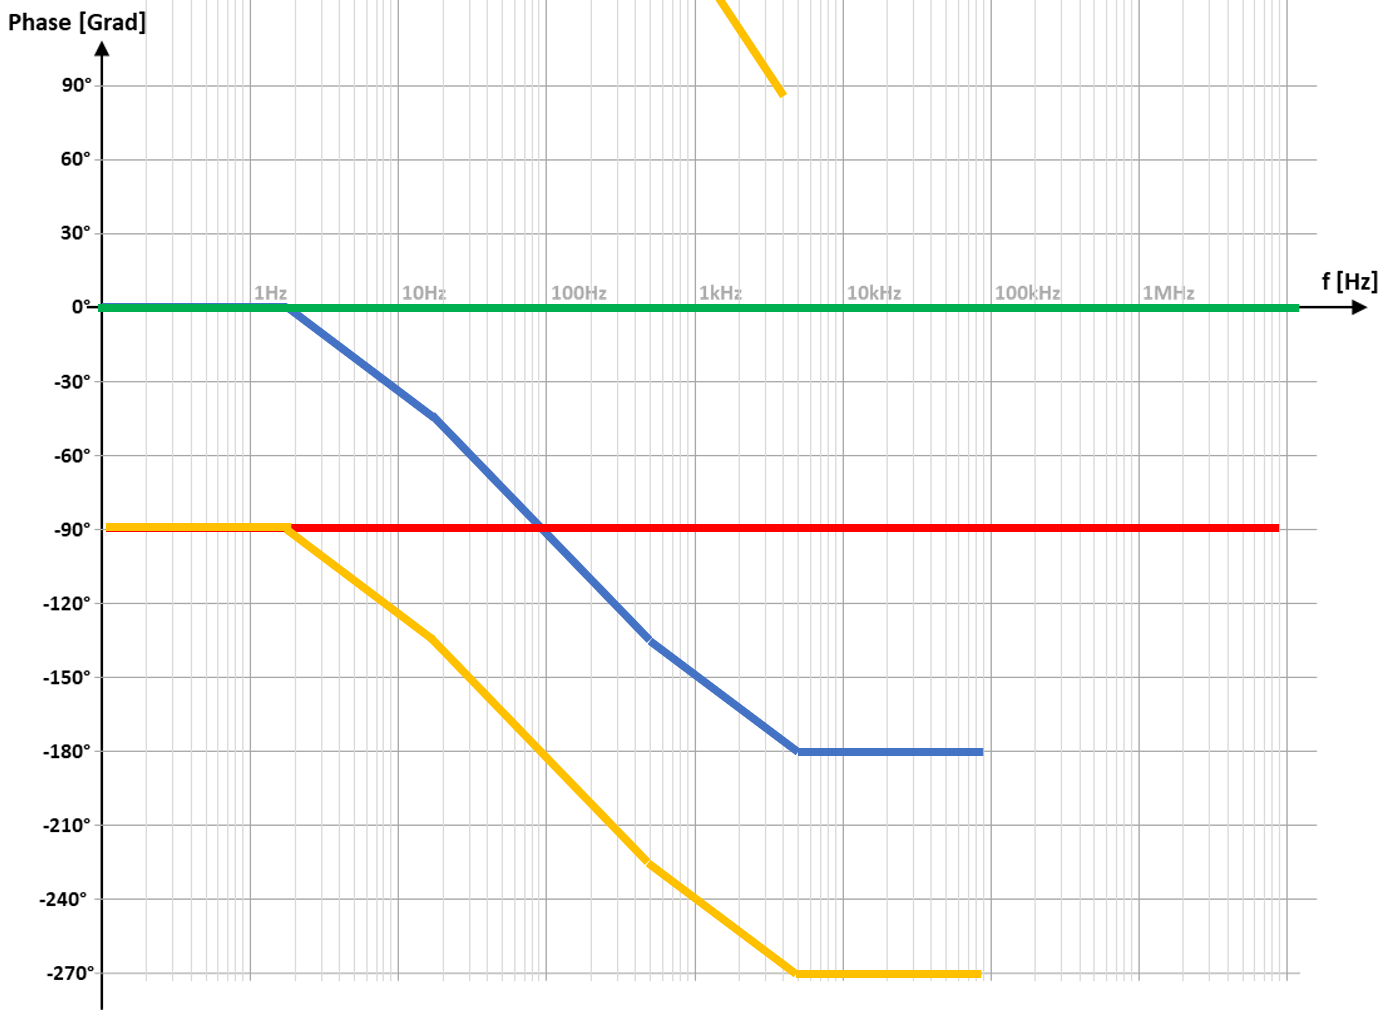
\includegraphics[width=1\linewidth, height=8cm]{img/Bode_08.png}
\end{figure}

\subsection{Rechteckspannung}
Nach dem Anlegen einer Rechteckspannung konnte festgestellt werden, dass die Ausgangsspannung sehr linear ansteigt und den maximalen Wert der Eingangsspannung leicht übersteigt und sich anschließend auf diese einstellt.
\begin{figure}[h]
    \centering
    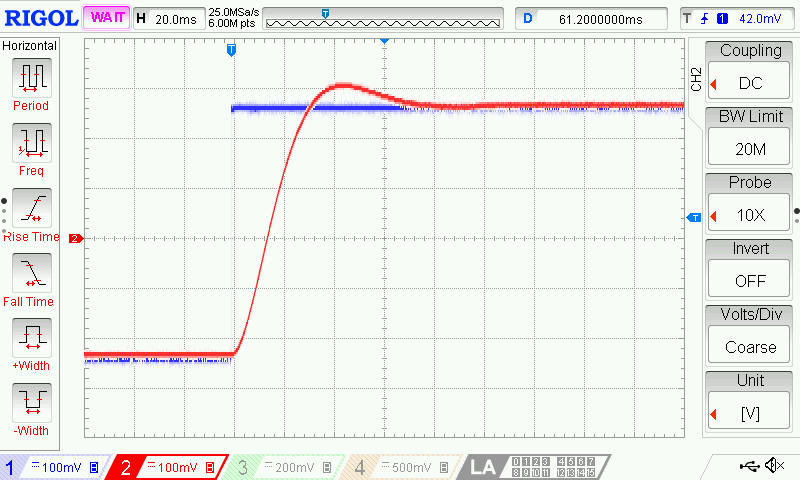
\includegraphics[width=0.8\linewidth]{img/Oszi_02.jpg}
\end{figure}

\subsection{Messung der Überschwingung}
Die Spannung der Überschwingung beträgt ca. 42 mV. Da die maximale Änderung der Eingangsspannung 500 mV beträgt, ergibt dies einen Überschwinger von 8.4 \%.
\begin{figure}[h]
    \centering
    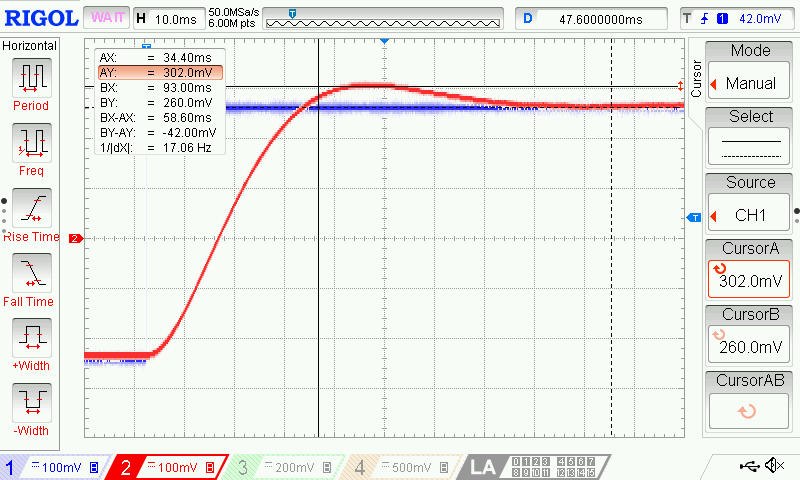
\includegraphics[width=0.8\linewidth]{img/Bode_03.jpg}
\end{figure}

\subsection{Dreieckspannung}
Beim Anliegen einer Dreiecksspannung wurde beobachtet, dass bei einer geringen Signalfrequenz die Ausgangsspannung ungefähr gleich der Eingangsspannung ist.\\
\begin{figure}[h]
    \centering
    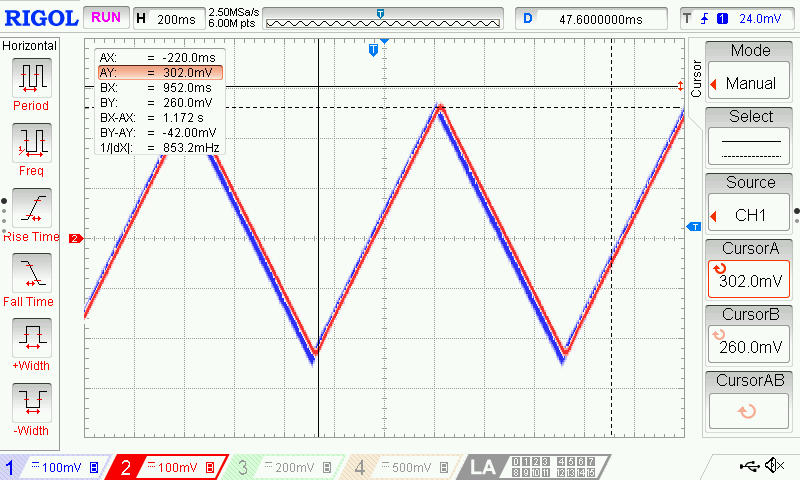
\includegraphics[width=0.85\linewidth]{img/Oszi_04.jpg}
\end{figure}\\
Wenn jedoch die Signalfrequenz erhöht wird, ähnelt die Form des Ausgangssignals einem Sinus.
\begin{figure}[h]
    \centering
    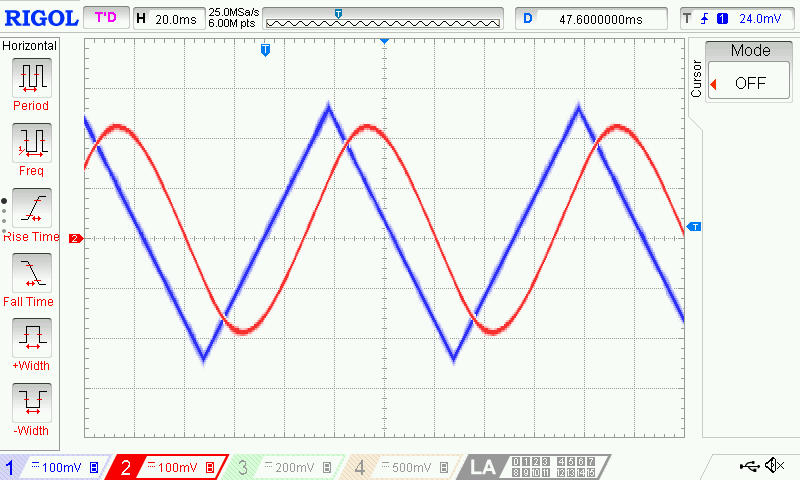
\includegraphics[width=0.85\linewidth]{img/Oszi_05.jpg}
\end{figure}


\end{document}
